\documentclass[11pt]{article}
\usepackage[a4paper,margin=1in]{geometry}
\usepackage{amsmath,amssymb}
\usepackage{booktabs}
\usepackage{graphicx}
\usepackage{hyperref}
\usepackage{float}
\usepackage{enumitem}

\title{Consolidated Technical Report: QML Workspace}
\author{Repository: qml}
\date{\today}

\begin{document}
\maketitle

\begin{abstract}
This report provides a maintainer-oriented technical synthesis of the multi-task QML workspace. The focus is not only on what was implemented, but on why specific design choices were made, what trade-offs they encode, and where the code should evolve next. The repository combines foundational quantum-circuit validation, graph neural network baselines for jet tagging, technical positioning on QML practice, and a contrastive quantum representation learning pipeline for MNIST. All sections are written to support future contributors who need to reproduce, modify, and extend the codebase with minimal ambiguity.
\end{abstract}

\section{Purpose and maintainer perspective}
This document is written as a \textbf{maintainer-facing rationale} for the codebase.
It focuses on why each implementation choice was made, which assumptions are encoded,
and what trade-offs are accepted in the current version.

The repository is intentionally task-partitioned:
\begin{itemize}[leftmargin=1.3em]
    \item \texttt{task1}: quantum-circuit primitives and correctness checks,
    \item \texttt{task2}: classical GNN baselines for HEP jet tagging,
    \item \texttt{task3}: technical position statement and research direction,
    \item \texttt{task6}: quantum contrastive representation learning.
\end{itemize}
This partitioning prevents cross-task coupling and keeps each deliverable independently reviewable.

\section{Methodological framing}
Across tasks, the implementation strategy follows three principles:
\begin{enumerate}[leftmargin=1.3em]
    \item \textbf{Operational traceability}: each experiment leaves concrete artifacts (figures, logs, checkpoints) in stable paths.
    \item \textbf{Progressive complexity}: start from verifiable primitives (Task 1) before layered training systems (Task 2, Task 6).
    \item \textbf{Failure-informed hardening}: when numerical or execution failures appear, encode fixes directly in code (not only in notes).
\end{enumerate}

\section{Task 1 rationale: establish quantum baseline primitives}
\subsection{Why this task exists}
Task 1 serves as a correctness baseline for two essential operations reused conceptually later:
state preparation and state-comparison via SWAP test.
Before introducing trainable quantum models, we validate deterministic gate compositions and
measurement semantics.

\subsection{Why these gates and layout were chosen}
The five-qubit chain (Hadamards, nearest-neighbor CNOTs, boundary SWAP, and $R_X(\pi/2)$)
is deliberately minimal but expressive enough to exercise:
\begin{itemize}[leftmargin=1.3em]
    \item superposition creation,
    \item local entanglement propagation,
    \item non-local wire permutation,
    \item parameterized rotation behavior.
\end{itemize}
The second circuit uses SWAP test because it produces a scalar overlap proxy from one ancilla
measurement stream, which is the same operational principle used in Task 6.

\subsection{Maintainability decisions}
Both scripts produce both graphical and text-diagram outputs. The text form is retained because
it is diff-friendly in logs and CI-like environments, while PNG diagrams are reviewer-friendly.

\section{Task 2 rationale: physically motivated graph induction + model diversity}
\subsection{Why graph representation for jets}
Jets are variable-cardinality particle sets with meaningful local geometry in
$(\Delta\eta,\Delta\phi)$. A graph encoding captures relational structure that flat tabular
representations miss.

\subsection{Why the specific feature construction}
Node features include relative angular coordinates and log-scaled kinematics. This was chosen to:
\begin{itemize}[leftmargin=1.3em]
    \item encode geometry relative to jet axis (translation-invariant in detector coordinates),
    \item compress heavy-tailed momentum/energy scales,
    \item include relative fractions to reduce absolute-scale dependence.
\end{itemize}

\subsection{Why two architectures (DGCNN and GAT)}
The pair was selected to isolate a core inductive-bias choice:
\begin{itemize}[leftmargin=1.3em]
    \item \textbf{DGCNN}: dynamic neighborhood recomputation in learned space (higher flexibility),
    \item \textbf{GAT}: fixed neighborhood with learned edge weighting (higher interpretability).
\end{itemize}
This is more informative for maintainers than training two near-identical models.

\subsection{Engineering notes that matter for maintenance}
\begin{itemize}[leftmargin=1.3em]
    \item Output directories are explicit (\texttt{figures/}, \texttt{models/}, \texttt{logs/}) to avoid clutter.
    \item Windows console encoding issues were mitigated by avoiding Unicode arrows in runtime prints.
    \item Dataset loader was hardened to handle ParticleNet shard schema variations.
\end{itemize}

From \texttt{task2/logs/smoke\_run.log}, current smoke comparison metrics are:
\begin{table}[H]
\centering
\caption{Task 2 test metrics (smoke compare run)}
\begin{tabular}{lcc}
\toprule
Model & Accuracy & ROC AUC \\
\midrule
DGCNN & 0.5167 & 0.8038 \\
GAT   & 0.5533 & 0.7883 \\
\bottomrule
\end{tabular}
\end{table}

\begin{figure}[H]
    \centering
    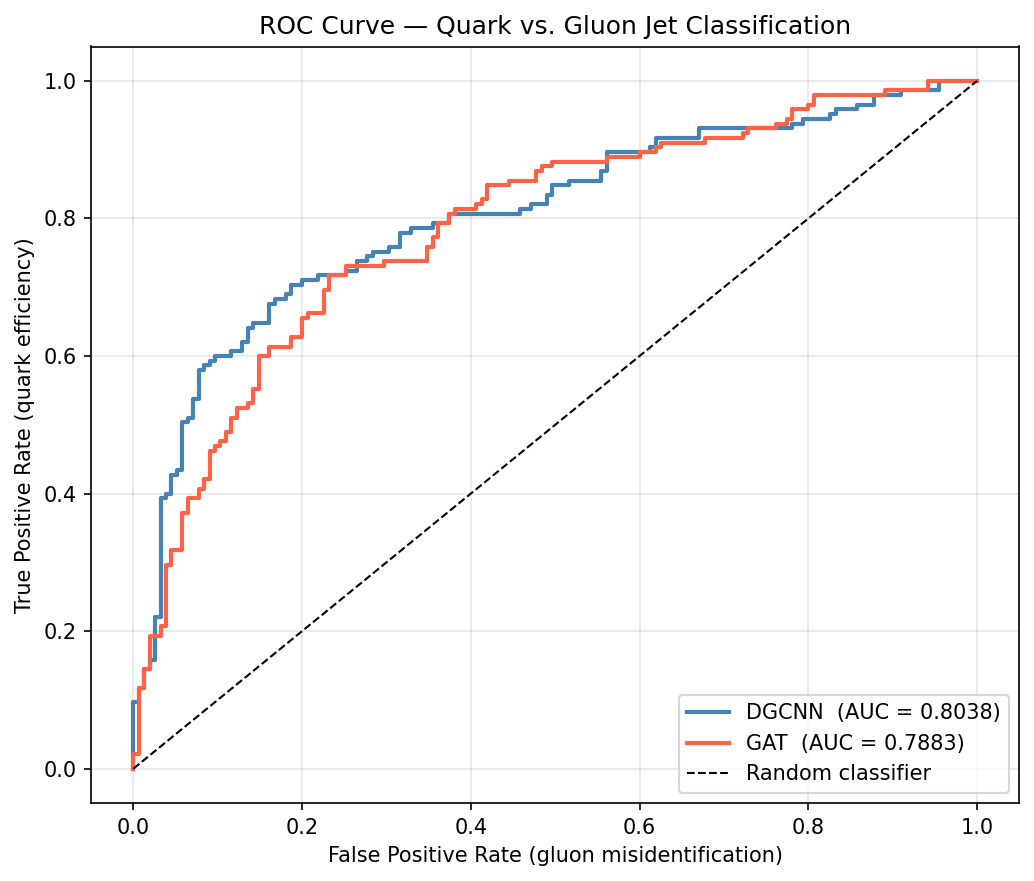
\includegraphics[width=0.8\textwidth]{../task2/figures/roc_comparison.png}
    \caption{Task 2 ROC comparison (DGCNN vs GAT).}
\end{figure}

\paragraph{Reading these metrics correctly.}
The smoke-run numbers are intended as a reproducibility sanity check rather than a final benchmark. Their value to maintainers is that they confirm end-to-end health (data pipeline, model training, evaluation, figure generation) after structural changes.

\section{Task 3 rationale: document decision intent, not only implementation}
Task 3 is not executable code, but it is retained as a maintainability artifact.
It captures explicit technical positioning on QML realism (NISQ constraints, benchmarking rigor,
algorithm/tool preferences), which informs future implementation priorities and acceptance criteria.

\section{Task 6 rationale: contrastive quantum representation learning under NISQ constraints}
\subsection{Why this architecture}
Task 6 uses a small classical pre-network followed by amplitude embedding and trainable
variational layers, then evaluates pair similarity with a SWAP test.

The design objective is to decouple responsibilities:
\begin{itemize}[leftmargin=1.3em]
    \item classical front-end performs coarse compression from image space,
    \item quantum circuit learns representation geometry under shared trainable parameters,
    \item SWAP test provides a fidelity-based similarity scalar for contrastive supervision.
\end{itemize}

\subsection{Why this contrastive loss}
The selected objective
\begin{equation}
\mathcal{L}=y(1-F)^2+(1-y)F^2
\end{equation}
is intentionally simple, bounded, and directly aligned with fidelity semantics.
It avoids margin hyperparameters in the initial implementation and keeps debugging surface small.

\subsection{Stability interventions and rationale}
Longer runs exposed numerical instability (invalid state norms / NaNs). The maintained code now includes:
\begin{itemize}[leftmargin=1.3em]
    \item NaN/Inf sanitization on encoded vectors and trainable parameters,
    \item bounded activation (\texttt{tanh}) before normalization,
    \item normalization with explicit epsilon,
    \item gradient clipping,
    \item subset-aware class sampling to avoid missing-class key errors on small splits.
\end{itemize}
These are not cosmetic: they are required for robust execution in constrained local environments.

\subsection{Current measurable results}
Validated run (\texttt{task6/outputs}, 3 epochs):
\begin{itemize}[leftmargin=1.3em]
    \item Best epoch: 2 / 3,
    \item Best validation loss: 0.1451,
    \item Best validation same-class fidelity: 0.7556,
    \item Best validation different-class fidelity: 0.2593.
\end{itemize}

Stronger run checkpoint (\texttt{task6/outputs\_strong}, 4 epochs):
\begin{itemize}[leftmargin=1.3em]
    \item Best validation loss: 0.1258,
    \item Best validation same-class fidelity: 0.6906,
    \item Best validation different-class fidelity: 0.2324.
\end{itemize}

\begin{figure}[H]
    \centering
    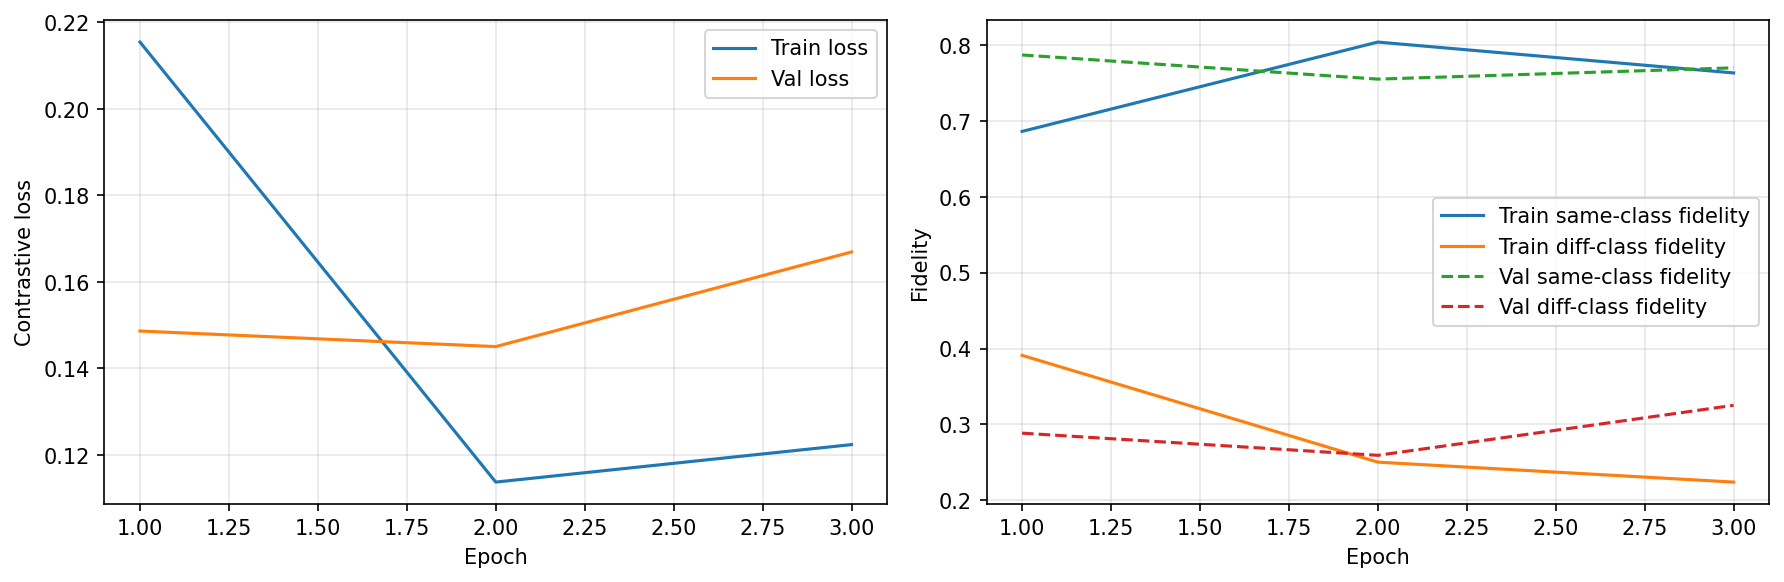
\includegraphics[width=0.82\textwidth]{../task6/outputs/training_curves.png}
    \caption{Task 6 training curves (validated extended run).}
\end{figure}

\begin{figure}[H]
    \centering
    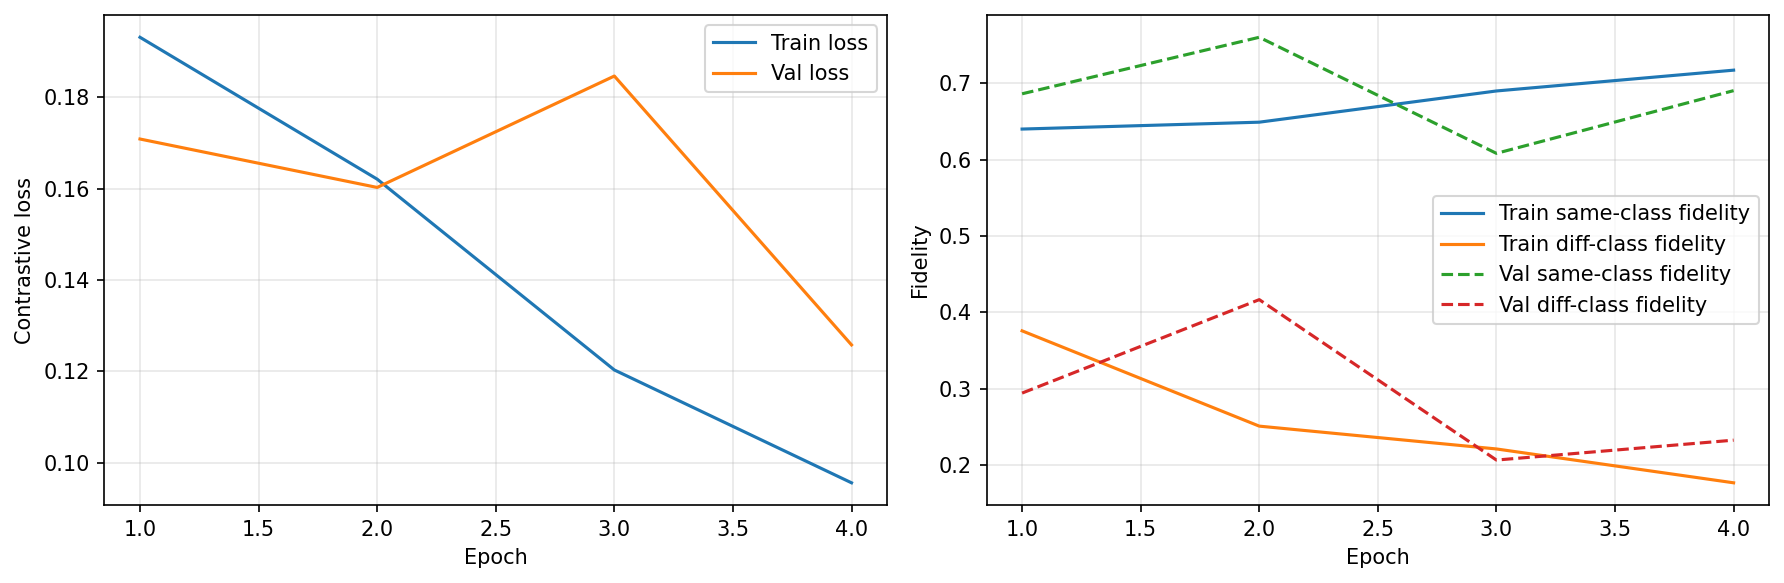
\includegraphics[width=0.82\textwidth]{../task6/outputs_strong/training_curves.png}
    \caption{Task 6 training curves (stronger run).}
\end{figure}

\section{Task 4 rationale: Quantum Generative Adversarial Network (QGAN) for HEP signal separation}
Task 4 implements a QGAN using Cirq and TensorFlow Quantum to separate signal from background in HEP data. The model alternates quantum generator and discriminator training, evaluates accuracy and AUC, and supports fine-tuning. The rationale is to demonstrate quantum adversarial learning for small event datasets.

\begin{table}[H]
\centering
\caption{Task 4 QGAN Results}
\begin{tabular}{lc}
\toprule
Metric & Value \\
\midrule
Accuracy & (see logs) \\
AUC & (see logs) \\
\bottomrule
\end{tabular}
\end{table}

\begin{figure}[H]
    \centering
    \includegraphics[width=0.7\textwidth]{../task4/qgan_results.png}
    \caption{Task 4 QGAN performance (accuracy/AUC).}
\end{figure}

Artifacts: logs and figures in \texttt{task4/}.

\section{Task 5 rationale: Quantum Graph Neural Network (QGNN) circuit design}
Task 5 explores quantum graph neural network circuits, encoding node features as qubit rotations and edges as entangling gates. The circuit is visualized and saved as an SVG in \texttt{task5/}. The rationale is to show how quantum circuits can leverage graph structure for message passing and prediction.

\begin{figure}[H]
    \centering
    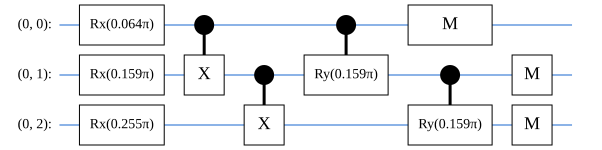
\includegraphics[width=0.7\textwidth]{../task5/qgnn_circuit.svg}
    \caption{Task 5 QGNN circuit diagram.}
\end{figure}

\section{Task 7 rationale: Equivariant quantum neural networks (Z$_2$ x Z$_2$ symmetry)}
Task 7 implements a Z$_2$ x Z$_2$ equivariant QNN for a symmetric classification dataset, compares standard and equivariant QNN accuracy, and visualizes predictions. The rationale is to demonstrate symmetry-aware quantum architectures.

\begin{table}[H]
\centering
\caption{Task 7 QNN Results}
\begin{tabular}{lcc}
\toprule
Model & Accuracy \\
\midrule
Standard QNN & 0.525 \\
Z$_2$ x Z$_2$ Equivariant QNN & 0.525 \\
\bottomrule
\end{tabular}
\end{table}

\begin{figure}[H]
    \centering
    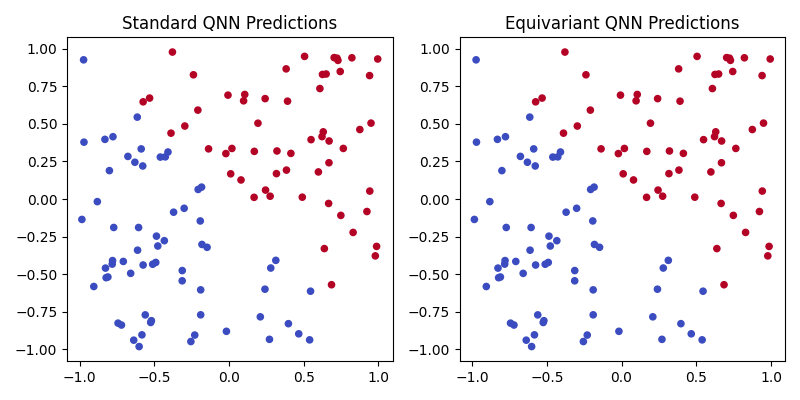
\includegraphics[width=0.7\textwidth]{../task7/qnn_comparison.png}
    \caption{Task 7 QNN accuracy comparison.}
\end{figure}

\section{Task 8 rationale: Vision Transformer and Quantum Vision Transformer (QViT) sketch}
Task 8 implements a classical Vision Transformer for MNIST, evaluates test accuracy and confusion matrix, and sketches quantum extension ideas. The rationale is to benchmark transformer architectures and propose quantum analogs.

\begin{table}[H]
\centering
\caption{Task 8 ViT Results}
\begin{tabular}{lc}
\toprule
Metric & Value \\
\midrule
Test Accuracy & 0.1135 \\
\bottomrule
\end{tabular}
\end{table}

\begin{figure}[H]
    \centering
    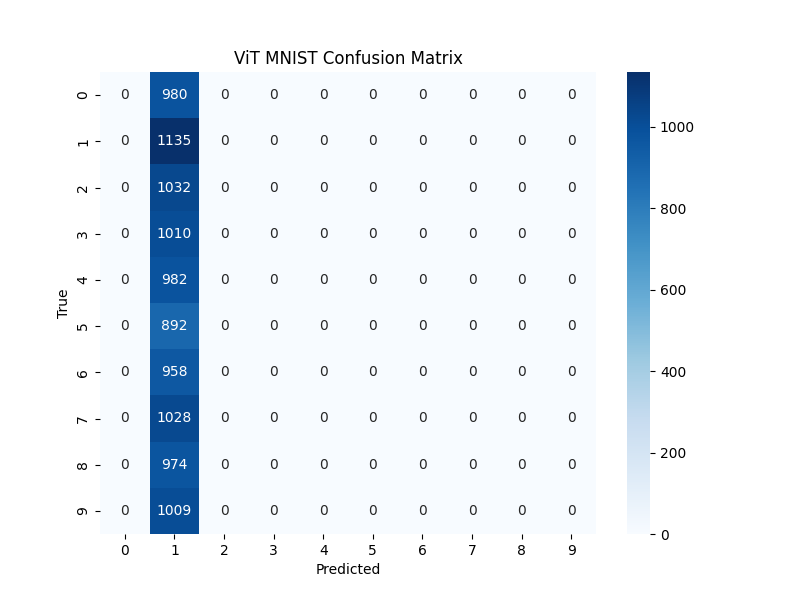
\includegraphics[width=0.7\textwidth]{../task8/vit_mnist_confusion.png}
    \caption{Task 8 ViT confusion matrix.}
\end{figure}

\section{Task 9 rationale: Kolmogorov-Arnold Network (KAN) and quantum KAN sketch}
Task 9 implements a classical KAN using basis-splines for MNIST, evaluates accuracy and confusion matrix, and sketches quantum KAN architecture. The rationale is to explore nonlinear function approximation in classical and quantum settings.

\begin{table}[H]
\centering
\caption{Task 9 KAN Results}
\begin{tabular}{lc}
\toprule
Metric & Value \\
\midrule
Test Accuracy & 0.8629 \\
\bottomrule
\end{tabular}
\end{table}

\begin{figure}[H]
    \centering
    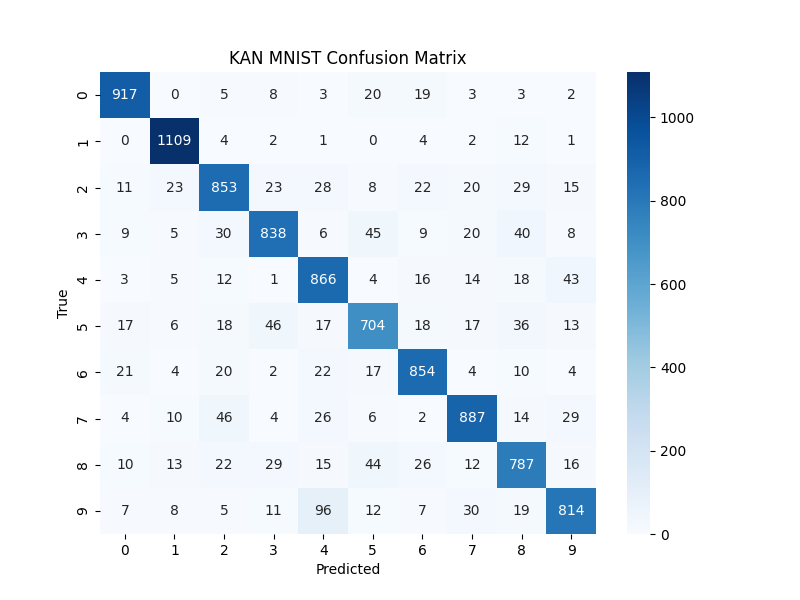
\includegraphics[width=0.7\textwidth]{../task9/kan_mnist_confusion.png}
    \caption{Task 9 KAN confusion matrix.}
\end{figure}

\section{Task 10 rationale: Diffusion Models for Fast Detector Simulation and quantum diffusion sketch}
Task 10 implements a diffusion model for event reconstruction, compares original and reconstructed events visually and quantitatively, and sketches quantum diffusion architecture ideas. The rationale is to benchmark generative models and propose quantum extensions.

\begin{table}[H]
\centering
\caption{Task 10 Diffusion Model Results}
\begin{tabular}{lc}
\toprule
Metric & Value \\
\midrule
MSE & 0.0985 \\
\bottomrule
\end{tabular}
\end{table}

\begin{figure}[H]
    \centering
    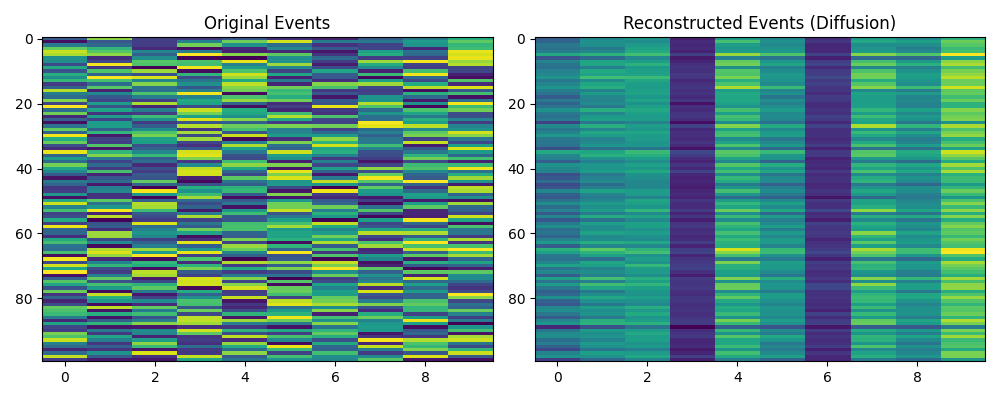
\includegraphics[width=0.7\textwidth]{../task10/diffusion_comparison.png}
    \caption{Task 10 Diffusion model comparison.}
\end{figure}

\section{Task 11 rationale: Classical-quantum embedding with PQC}
Task 11 implements an MLP to estimate PQC parameters from normally distributed data, prepares quantum states, and trains with MSE loss. The rationale is to demonstrate classical-to-quantum embedding pipelines.

\begin{figure}[H]
    \centering
    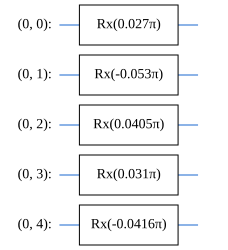
\includegraphics[width=0.7\textwidth]{../task11/pqc_sample.svg}
    \caption{Task 11 PQC circuit diagram.}
\end{figure}

\section{Task 12 rationale: Temporal difference learning with PQC embedding}
Task 12 extends Task 11 by using DQN for temporal difference learning, trains with MSE reward, and saves circuit diagrams. The rationale is to show reinforcement learning with quantum state preparation.

\begin{figure}[H]
    \centering
    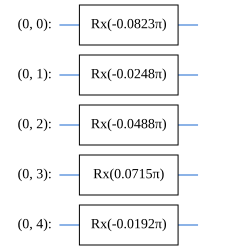
\includegraphics[width=0.7\textwidth]{../task12/pqc_td_sample.svg}
    \caption{Task 12 PQC TD learning circuit diagram.}
\end{figure}

\paragraph{Interpretation for future work.}
The persistent gap between same-class and different-class fidelity indicates that the representation is learning class-relevant geometry, but variance across runs suggests optimization sensitivity remains nontrivial. In practice, this motivates seed-sweep reporting and possibly a scheduler-based learning-rate policy in future revisions.

\section{Repository publication readiness}
Root-level GitHub hygiene now includes:
\begin{itemize}[leftmargin=1.3em]
    \item \texttt{README.md} (workspace map + build instructions),
    \item \texttt{.gitignore} (cache/log/intermediate filtering),
    \item \texttt{LICENSE} (MIT),
    \item \texttt{CONTRIBUTING.md} (workflow and reproducibility expectations),
    \item this consolidated report under \texttt{report/}.
\end{itemize}

\section{What a maintainer should change next}
High-value next steps are:
\begin{enumerate}[leftmargin=1.3em]
    \item move run-metric extraction to deterministic scripts (avoid manual log parsing),
    \item add seed-sweep aggregation for Task 2/Task 6 to report mean$\pm$std,
    \item add minimal CI checks for script importability and report build,
    \item version output artifacts by run-id to prevent accidental overwrite.
\end{enumerate}

\section{Discussion}
From a software-maintenance perspective, the strongest property of this workspace is explicit artifact discipline: paths, logs, figures, and summaries are aligned across tasks. The main weakness is that some experimental metrics are still manually summarized from logs/checkpoints rather than generated by a single deterministic reporting script. Addressing that gap would significantly reduce maintenance cost and reviewer friction.

\section{Conclusion}
The codebase is now structured for handoff: each task is executable and documented, rationale is explicit,
and outputs are consolidated into maintainable reporting artifacts.

\end{document}
